\documentclass{css}
%\documentclass[english]{css}

\usepackage[dvipdfmx]{graphicx}
\usepackage{latexsym}
\usepackage{listings}
\usepackage{url}
\urlstyle{same}
\usepackage{tikz}
\usetikzlibrary{arrows.meta}

\newcommand{\cssyear}[0]{2026}
\newcommand{\cssname}[0]{CSS 2026}
\newcommand{\cssversion}[0]{2026/06/01}
\newcommand{\cssemail}[0]{css2026-office@iwsec.org}

\makeatletter
\newcommand\newblock{\hskip .11em\@plus.33em\@minus.07em}
\makeatother

\begin{document}

%% 本文が和文の場合，タイトル・著者名・著者所属・概要は，和文・英文共に必須．

\title{脆弱性情報の上流は安定していない: \\ 公開前検査による116日間の全数観測}
\etitle{Vulnerability Feeds Are Not Stable: A 116-Day Exhaustive Observation via Pre-Publication Inspection}

\affiliate{FUTURE}{フューチャー株式会社\\
Future Corporation}

\author{篠原 俊一}{Shunichi Shinohara}{FUTURE}[s.shinohara.yx@future.co.jp]
\author{中岡 典弘}{Norihiro Nakaoka}{FUTURE}[n.nakaoka.46@future.co.jp]
\author{神戸 康多}{Kota Kanbe}{FUTURE}[k.kanbe.r4@future.co.jp]

\begin{abstract}
脆弱性データベースは多数の上流データソースを集約して構築されるが，上流は必ずしも安定せず，データの消失や公開済みアドバイザリの遡及的な書き換えが現実に起きている．
本研究では，この不安定性を定量観測するため，OSS脆弱性スキャナVulsのDB公開CIに公開前検査を実装した．
検査は公開候補と直前の公開版を，検知結果と検知条件構造の2観点で比較し，変動率が閾値を超えた場合は公開を保留して人間の確認に委ねる．
116日間の本番運用の全数調査では69件の独立イベントで検査が発動し，全工程を履歴管理する既報の基盤を用いて，その全てについて原因が上流データの変化か，変換やDB構築や取得設定といった自前の処理かを切り分けて特定できた．
日常変動と構造的イベントは変動率で桁が分離しており，閾値による単純な判定が実用になること，また欠損DBの公開を3回阻止したことを示す．
\end{abstract}

\begin{jkeyword}
脆弱性データベース，データ品質，公開前検査，履歴管理，ソフトウェアサプライチェーン
\end{jkeyword}

\begin{eabstract}
Vulnerability databases are built by aggregating many upstream data sources, but these upstreams are not always stable: data disappears, and published advisories are retroactively rewritten.
To quantify this instability, we implemented a pre-publication inspection in the CI pipeline that builds and publishes the database of Vuls, an open-source vulnerability scanner.
The inspection compares each publication candidate with the previously published version in terms of detection results and detection-criteria structure, and when the change rate exceeds a threshold, it withholds publication pending human review.
In an exhaustive study covering 116 days of production operation, the inspection fired on 69 independent events, and our previously reported infrastructure, which keeps every pipeline stage under version control, allowed us to attribute every event to either upstream data changes or our own processing such as data transformation, database construction and fetch configuration.
We show that everyday fluctuation and structural events are separated by an order of magnitude in change rate, making this simple threshold-based inspection practical, and that the inspection blocked the publication of defective databases three times.
\end{eabstract}

\begin{ekeyword}
Vulnerability Database, Data Quality, Pre-Publication Inspection, History Management, Software Supply Chain
\end{ekeyword}

\maketitle

\section{はじめに}
\label{sec:intro}

脆弱性対応の実務は，ディストリビュータやベンダが公開するアドバイザリや脆弱性フィードを「正」として組み立てられている．
脆弱性スキャナはこれらを集約した脆弱性データベース(以下，脆弱性DB)に依存し，検知結果はフィードの内容をほぼそのまま反映する．
ここには，上流フィードは概ね安定しており，変化は新規脆弱性の追加という単調な形をとる，という暗黙の仮定が置かれている．
この仮定はどの程度正しいのだろうか．

我々はOSS脆弱性スキャナVuls\cite{vuls}のエコシステムにおいて，40超のデータソースから脆弱性DB(vuls.db)をCIで自動ビルドし，6時間おきに公開している．
前稿\cite{nakaoka2025}では，この収集(fetch)，変換(extract)，構築(db build)の全工程をバージョン管理システムと連携させ，脆弱性情報の変更履歴を客観的事実として追跡・再現可能にする履歴管理基盤を報告した．
本稿はその続編にあたる．
前稿の基盤が「脆弱性情報の変化を\textbf{記録できる}」ことを示したのに対し，本稿はその記録能力を使って「上流は実際に\textbf{どう変化しているか}」を系統的に測定し，さらにその測定をDBの公開品質管理として実用化した結果を報告する．

測定の装置は単純である．
公開直前の候補DBを，現に公開されている直前版(baseline)と自動比較し，変動率が閾値を超えたら公開を保留して人間に見せる．
我々はこれを\textbf{公開前検査}(diff guard)と呼ぶ．
導入の直接の動機は，自らのパイプライン変更と上流の破損データの複合，およびDBとスキャナのバージョン非互換によって「壊れたDB」を公開してしまった2件のインシデント(\ref{sec:incidents}節)であり，検査は第一義には安全ネットである．
しかし116日間の本番運用で得られた発動記録の全数調査は，副産物として，脆弱性情報の上流がいかに大きく，頻繁に，時に黙って動くかの縦断観測データとなった．

本稿の貢献は次の3点である．

\begin{enumerate}
\item \textbf{上流不安定性の実測}(\ref{sec:results}節，\ref{sec:discussion}節):
116日間・943 runの全数調査により，上流フィードの不安定性を69件の独立イベントとして分類・定量化した．
観測されたイベントは，可用性の不安定(月次データの消失とフラッピング)，完全性の危うさ(遡及的な再キュレーションやアナウンスのないサーバ側再編)，スケールの分布(日常変動と構造的イベントの桁分離)の3群に整理できる．
これらの上流は他の脆弱性ツール(Trivy，Grype，OSV系等)も共有しており，知見はエコシステム横断で再利用可能である．
\item \textbf{原因帰属の方法論}(\ref{sec:method}節):
発動の原因をビルダ，抽出器，取得設定，上流の順に容疑を除外して確定する切り分け手順を定義し，全イベントに適用した．
各ステップは履歴管理基盤\cite{nakaoka2025}の対応する工程の履歴(DBメタデータ，抽出器のコミット履歴，rawデータのGit差分)に依拠しており，全工程の履歴管理が帰属の成立条件であることを示す．
\item \textbf{公開前検査の設計と運用機構}(\ref{sec:design}節):
検知結果差分とDB構造差分の2観点による検査本体に加え，監査証跡付き手動override(promote)，対象別閾値の統計的導出と定期的な再導出(grooming)という，検査を運用し続けるための機構を設計・実装した．
検査は欠損DBの公開を3回阻止した．
\end{enumerate}

\begin{figure}[tb]
\centering
\begin{tikzpicture}[font=\footnotesize, >=Stealth,
  b/.style={draw, rounded corners=1pt, align=center, inner sep=3pt, minimum height=5mm},
  hist/.style={b, fill=gray!15},
  lbl/.style={font=\scriptsize, text=black!70},
  note/.style={font=\scriptsize, text=black!60, align=left}]
  \node[b]    (up)   at (0,0)     {上流データソース(40+)};
  \node[hist] (raw)  at (0,-0.95) {raw(Git履歴)};
  \node[hist] (ext)  at (0,-1.9)  {extracted(Git履歴)};
  \node[hist] (cand) at (0,-2.85) {候補DB(digestのみでpush)};
  \node[b, fill=orange!20] (g) at (0,-3.8) {公開前検査(Dn / Do / DB)};
  \node[b]    (pub)  at (-1.7,-4.9) {GHCRタグ公開};
  \node[hist] (hold) at (1.8,-4.9)  {保留(タグなしdigest)};
  \draw[->] (up) -- (raw)   node[midway,left,lbl] {fetch};
  \draw[->] (raw) -- (ext)  node[midway,left,lbl] {extract(抽出器)};
  \draw[->] (ext) -- (cand) node[midway,left,lbl] {db build(ビルダ)};
  \draw[->] (cand) -- (g);
  \draw[->] (g) -- (pub)  node[midway,left,lbl]  {PASS};
  \draw[->] (g) -- (hold) node[midway,right,lbl] {FAIL};
  \draw[->] (hold) -- (pub) node[midway,below=5pt,lbl] {人間レビュー後promote};
  \draw[->, dashed] (pub.west) .. controls +(-0.75,0.3) and +(-1.3,-0.1) .. (g.west)
    node[pos=0.45,left,lbl,align=center] {baseline\\(直前公開版)};
  \node[note] (n1) at (3.35,-0.95) {上流確定};
  \node[note] (n2) at (3.35,-1.9)  {抽出器除外};
  \node[note] (n3) at (3.35,-2.85) {ビルダ除外};
  \node[note, align=center] at (3.35,-0.2) {原因帰属(\ref{sec:method}節)\\が参照};
  \draw[densely dotted] (raw.east)  -- (n1.west);
  \draw[densely dotted] (ext.east)  -- (n2.west);
  \draw[densely dotted] (cand.east) -- (n3.west);
\end{tikzpicture}
\caption{脆弱性DB公開パイプラインと公開前検査．全工程がGit履歴管理\cite{nakaoka2025}され，原因帰属(\ref{sec:method}節)は各工程の履歴を参照する．}
\label{fig:arch}
\end{figure}

\section{背景}
\label{sec:background}

\subsection{履歴管理基盤(前稿)の要点}
\label{sec:infra}

vuls.dbの生成は3工程からなる\cite{nakaoka2025,vuls-data-update,vuls-data-db}．
fetch工程は一次情報源から取得したデータを原形をほぼ保ったvuls-data-raw形式で，extract工程はそれを共通スキーマのvuls-data-extracted形式で，それぞれGit管理下に置く．
db build工程はextractedデータからBoltDB形式のvuls.dbを構築し，コンテナレジストリ(GitHub Container Registry，以下GHCR)にタグおよびdigestで公開する．
以下本稿では，extract工程の変換コードを\textbf{抽出器}，db build工程の構築コードを\textbf{ビルダ}と呼ぶ．
この構成により，(1)任意時点の上流データの状態をコミット単位で遡れる，(2)DBをdigestで固定して検知結果を再現できる，という2つの性質が得られている．
本稿の測定はこの2性質の直接の応用である．

\subsection{動機となった2つのインシデント}
\label{sec:incidents}

2026年3月，生成物としてのDBが壊れているのに公開が成功してしまう事象を2件経験した．

\textbf{インシデント1(RHEL VEX，false negative)}:
我々がパイプラインにデータ形式変更を投入したのと同じ日に，上流から不正なVEX(Vulnerability Exploitability eXchange)データが配信された．
変換はエラー終了してデータが旧形式のまま残り，新形式を前提とする後段フィルタが空データを生成した．
結果，redhat:9で本来検知されるべきCVEの51.9\%(3,387件)が「影響なし」となるDBが公開された．
どちらか一方だけなら実害はなかった: 不正データがなければ変換は新形式へ移行して整合し，形式変更がなければ変換失敗はデータが一時的に古いままになるだけで済んだ．
工程間の形式整合を欠いた我々の実装と上流の異常が複合して初めて成立した欠陥である．

\textbf{インシデント2(Ubuntu \texttt{vulnerable: false}，false positive)}:
DB側に導入されたマーカを，それを解釈するフィルタを持たない旧バージョンのスキャナが読んだ結果，ubuntu\_2204の検知件数が5,968件から12,296件(+106.0\%)に倍増した．
DB単体でもスキャナ単体でも正常であり，組み合わせの非互換が原因である．

従来のCIが検査するのはビルドの成否であって，生成物のデータとしての妥当性ではない．
また2件は対照的で，前者はDB単体を見れば検出できるが，後者はDBとスキャナ(の特定バージョン)の組で実行しなければ検出できない．
この2面性が次章の設計に直結する．

\section{公開前検査の設計}
\label{sec:design}

\subsection{導入前ベンチマーク: 閾値検査の成立可能性}
\label{sec:benchmark}

脆弱性DBは日々更新されるため差分ゼロはあり得ず，閾値による検査が成立するには正常な変動と異常なイベントが変動率で分離する必要がある．
導入前に，GHCR上に履歴として残っている過去37日分のDB(2026-02-15から03-29)を用い，連続1日ペア35組でDB構造差分を実測した．
通常運用の変動率は中央値0.3\%，最大6.2\%に収まり，期間中に10\%を超えた2組はいずれも実在の上流データ品質イベント(Red Hat VEX構造変更でredhat:6が65.1\%，SUSE OVAL大規模更新で12から16\%)であった．
正常帯と異常イベントが桁で分離するというこの観測が，閾値検査成立の根拠である．
なお，過去任意時点のDBペアでこの種のベンチマークが実行できること自体，公開物がdigest付きで履歴化されている\cite{nakaoka2025}ことの恩恵である．

\begin{figure}[tb]
\centering

\includegraphics[width=\linewidth]{./figures/fig2-benchmark.pdf}
\caption{導入前ベンチマーク: 連続1日ペア35組の最大変動率(対数軸)．破線はdb既定閾値10\%．橙の2ペアが実在の上流イベント(Red Hat VEX構造変更65.1\%，SUSE OVAL再発行16.1\%)であり，正常帯(中央値0.3\%)と桁で分離する．}
\label{fig:benchmark}
\end{figure}

\subsection{3つのチェック}
\label{sec:checks}

公開CIの圧縮後・公開前に，次の3チェックを実行する(検知結果差分の2つをDn(新スキャナ)とDo(旧スキャナ)，DB構造差分をDBと略記する)．

\begin{itemize}
\item \textbf{Dn: 検知結果差分(スキャナ最新版)}．
baselineとtargetの両DBに対して同一のスキャン結果fixture群(実機スキャン由来，数十ファイル)でスキャナを実際に実行し，ファイル単位で検知CVE集合を比較する．
変動率は(追加数+削除数)/baseline検知数で定義する．
\item \textbf{Do: 検知結果差分(固定した旧バージョンのスキャナ)}．
過去バージョンとの組でのみ現れる非互換退行(インシデント2型)を捕捉する．
\item \textbf{DB: DB構造差分}．
BoltDBを直接開き，ecosystem(後にソース単位へ細分化)ごとに検知条件木をleaf Criterionレベルまで平坦化して構造比較する．
スキャン結果もスキャナも不要でDBのみで完結する．
比較粒度をバイト列ではなくCriterionにしたのは，JSONキー順などの無害な変更での偽陽性を避けつつ，分母(全体で約330万Criterion)を大きく取り正常変動を小さなdriftとして吸収するためである．
\end{itemize}

チェック結果は変動率，増減の内訳，変動したCVEやアドバイザリのIDを含む構造化されたレポートとして常にCIのJob Summaryに出力される．
これは前稿が課題として挙げた「行ベース差分ではなく論理的な構造としての差分提示」\cite{nakaoka2025}の，公開品質管理という文脈での実装形でもある．
導入当初は最初のFAILで検査が停止する実装だったが，先にFAILしたチェックが後段のシグナルを隠す問題が判明し，現在は3チェックすべてを実行してから集約判定する．

\subsection{FAIL時の運用: 監査証跡付き手動promote}
\label{sec:promote}

候補DBは検査実行前にdigestのみ(タグなし)でGHCRにpushしておき，PASS時にのみタグを付けて「公開」する．
FAILした場合，候補はタグなしのままdigestで取得可能な状態で残るため，事後検証が可能である．
オペレータがレポートを確認し正当な変更と判断した場合は，専用workflowで該当digestに手動でタグ付けする(promote)．
実行者，digest，タグがrun履歴に残り，「誰が何を根拠にoverrideしたか」が追跡できる．
運用ルールとして，promoteの判断・実行は人間に限定している(調査を支援するAIエージェントには実行させない)．

\subsection{閾値のper-target / per-source化とgrooming}
\label{sec:threshold}

閾値はデフォルトでdetection 5\% / db 10\%とし，運用実績に基づき対象別に緩和するoverride機構を持つ．
導入1ヶ月の運用で，新ディストリビューション立ち上がり期の一括triage，rolling release，ベンダ月次サイクルといった反復的な正当変動が毎回検査に引っかかることが判明したためである．
override値は失敗履歴の統計から「観測ピーク+ヘッドルーム」で導出し，単発スパイクはoverrideせずFAILさせて人間に見せる(例: EOLディストリビューションが39\%動くのは異常として意図的に残置)．
リストの陳腐化を防ぐため約2ヶ月周期で全再導出する(grooming)．
さらに運用後期，ecosystem一括の変動率では大きなソースがノイズフロアになって小さなソースの異常を希釈する問題が顕在化し(\ref{sec:scaledist}節)，閾値もレポートもソース単位に細分化した．

\section{測定方法論: 全数調査と原因帰属}
\label{sec:method}

\textbf{全数調査}:
本番導入(2026-04-23)から08-16までの116日間，2系統(安定版 / 開発版)の全943 runを対象に，runログ，PR，promote履歴をGitHub APIで全数収集した．
FAIL中はpromoteがあるまでbaselineが動かず，同じ差分で6時間おきのcronが再FAILし続けるため，run数は重複を含む．
そこで連続FAILを1つに潰したfail sequence(104件)，さらに2系統を束ねソース単位の出現時系列で分解したsource-episode(\textbf{69件})を独立イベントの単位として定義した．

\textbf{原因帰属}:
各イベントについて，次の順で容疑を除外して原因を確定する．

\begin{enumerate}
\item \textbf{ビルダ除外}: baselineとtargetの両DBのメタデータに記録されたビルダのバージョンを比較する．一致すればDB構築コードは無罪．
\item \textbf{抽出器除外}: 対象期間の抽出器リポジトリのコミット履歴を走査する．当該ソースのfetch / extractコードに変更がなければ変換コードは無罪．
\item \textbf{取得設定除外}: 同期間のvuls-data-db(取得設定を持つリポジトリ)のコミットを走査する．取得対象のseedリストや新規データソースの追加がなければ取得設定は無罪．
\item \textbf{上流確定}: rawデータのGit履歴から対象期間のコミットを特定し，差分の中に変動と件数・IDが一致する変更実体(smoking gun．例えば新規アドバイザリファイル群やディレクトリの消失)を突き止める．
\end{enumerate}

この手順の各ステップは，履歴管理基盤\cite{nakaoka2025}の対応する工程の履歴にそれぞれ依拠している．
ビルダ除外はDBメタデータ，抽出器除外はコードのコミット履歴，上流確定はrawおよびextractedデータのGit履歴である．
全工程が履歴化されていなければ，例えば「上流の一時障害なので候補を破棄すべき」と「正当な変更なのでpromoteしてよい」の区別(\ref{sec:prevented}節)は当て推量になる．
逆に言えば，履歴管理は本測定の成立条件であり，前稿の基盤の実証でもある．
実際，全69イベントで帰属は完了し，「原因不明」は残らなかった．
ただし証拠の水準は一様ではない．
前半の観測窓と，後半窓で非上流と判定したイベント(取得設定由来2件と抽出器由来2件)については，原因となったコミットやPRの差分を直接の証拠として特定している．
後半窓で上流由来と判定したイベントは，ビルダ，抽出器，取得設定の3者をコミット履歴の走査で除外した上での帰属であり，raw差分のsmoking gunまで確認したのは代表事例に限られる．
また帰属手順は再現可能なtriage手順書として整備してチームで共有しており，AIエージェント用のスキルとしても記述している．実運用では一次調査をAIエージェントが実施し，人間がその報告を検証した上でpromoteの可否を判断する(\ref{sec:promote}節)．

\section{運用結果}
\label{sec:results}

\subsection{規模と原因分布}
\label{sec:scale}

943 run中，失敗は476 run．うち420 runが検査のステップで失敗した(閾値超過418+検査内インフラ障害2)．
独立イベントは69 source-episodeである．
原因の分布を表\ref{tab:attribution}に示す．
抽出器由来，取得設定由来，および公開を阻止した事例は原因のコミットや上流イベントまで個別に特定できており，残る発動は全て上流由来の正当な変更である．

\begin{table}[tb]
\caption{原因帰属の分布(事例単位)．$\dagger$は公開を阻止した判定．非上流由来の事例は全て原因のコミットまで特定済みで件数が確定する．残る発動は全て上流由来の正当な変更であり，fedora:46のような小規模baseline起因の構造的FAILを含む．}
\label{tab:attribution}
\centering
\small
\setlength{\tabcolsep}{4pt}
\begin{tabular}{lll}
\hline
判定 & 件数 & 代表例 \\
\hline
上流由来(a) 正当な変更 & 残り全て & 月次パッチ等 \\
上流由来(b) 一時的障害$\dagger$ & 2 & CVRF消失 \\
上流由来(c) 恒久的品質イベント & 2 & errata再編 \\
抽出器由来(コードバグ)$\dagger$ & 1 & 非決定的出力 \\
抽出器由来(意図的変更) & 3 & 検知の補完 \\
取得設定由来 & 2 & seed追加，新ソース \\
ビルダ由来 & 0 & (事例無し) \\
\hline
\end{tabular}
\end{table}

観測期間の後半では，非上流由来のイベントが4件発生した．
2件は前半に存在しなかった\textbf{取得設定由来}である．
我々自身が取得対象のseedリストを拡張した直後(2026-08-05から08-06，Windows更新プログラム(KB)のseed登録)にmicrosoft/microsoft-msucが211.3\%で発動し，新規データソースを追加した直後(08-10)にはmicrosoft/microsoft-servicingがbaseline不在のため100.0\%で発動した．
上流にも抽出器にも変更はなく，「何を取りに行くか」の設定変更が原因であり，帰属手順にvuls-data-db側のコミット走査(\ref{sec:method}節の手順3)を加えることで初めて分離できた．
残る2件は\textbf{抽出器由来の意図的変更}の再来である．
代表例では，2012年から2022年の履歴的アドバイザリに検知を補完する抽出器変更(検知を持つファイルが643件から1,065件に増加)のマージ直後に，cpe\_fortinet/fortinet-cvrfが135.5\%で発動した．
こちらは既存の抽出器コミット走査(同節の手順2)で特定できる．

\begin{figure*}[tb]
\centering

\includegraphics[width=\textwidth]{./figures/fig3-timeline.pdf}
\caption{116日間の発動タイムライン(source-episode 69件)．横棒は各episodeの持続期間(FAIL初出から終端まで)，点線はoverride導入時点(seed: 初期シード，snap: ubuntu:snap，windows: windows系detection，rocky: rocky\_10，per-source: ソース単位化，grooming: 2026-08のoverride再導出)．per-source化後のcpe\_*系はcpe行に含めた．}
\label{fig:timeline}
\end{figure*}

\subsection{実害を防いだ3事例}
\label{sec:prevented}

\begin{enumerate}
\item \textbf{Microsoft CVRF月次データ全消失(2回)}(CVRF: Common Vulnerability Reporting Framework):
上流APIが当月分のセキュリティ更新ドキュメント(700から1,300ファイル)を丸ごと返さなくなり，Windows系13ターゲットで最大53.6\%の削除のみの差分が発生した．
公開されていればインシデント1と同型の大量false negativeである．
検査は候補を破棄させ，上流回復後の再実行のみで復旧した．
raw履歴上，当月ファイル数は1273 $\rightarrow$ 0 $\rightarrow$ 1273 $\rightarrow$ 0 $\rightarrow$ 1278とフラッピングしており，単発の取得失敗ではなく上流配信自体の不安定であった(フラップの各時点がコミットとして残っているため，この認定自体が履歴管理の産物である)．
\item \textbf{AlmaLinux errataの縮退}:
errataフィードが1週間に複数回再編成され，アドバイザリ数が279から一時60まで減少，削除されたアドバイザリが参照するCVEの87\%(376件)が消失し，残存アドバイザリでもkernel更新の検知条件が73から2パッケージへ縮退した(変動率は縮退時99.2\%，後述の巻き戻し時に最大428.3\%)．
過去バージョン系列に対する大量のfalse negativeに直結する．復旧作業の過程で縮退DBは数時間公開に達したが，取り込みを縮退前のコミットにピン留めして同日中に巻き戻し，以後の流入を停止した．
その後，上流のHTML indexに残るのにフィードから消えたアドバイザリだけを自らの取得履歴のスナップショットからfetch時に復元する機構を組み込んだ上でアンピンした．
ピン留めも履歴からの復元も，取り込みが履歴管理されているから可能な操作である(原因は\ref{sec:integrity}節)．
\item \textbf{(限定的)VulnCheck一斉ロールアウト}:
単一コミットで145,672ファイル，+957万行という生成CPE(Common Platform Enumeration)設定の一斉付与をDBチェックが検出した．
ただし当時のecosystem一括の変動率では「cpe 28.9\%」としか言えず，候補はpromoteされた．
事後のソース単位の再分析で，当該ソース単独では189.6\%の変動であり，かつ実検知が60から75\%消失する退行を含んでいたことが判明した．
この教訓がソース単位への細分化(\ref{sec:threshold}節)の直接の動機である．
「発動したが分解能不足で判定を誤りかけた」事例として記録する．
\end{enumerate}

\subsection{false positive論と運用ループ}
\label{sec:fp}

発動の大半は正当な上流変更であり，これを「誤報」と見るかは設計思想による．
本検査は安全ネットであり，822 CVEを単一アドバイザリに同梱するカーネル更新や，約600パッケージを束ねた単一アドバイザリ(5,312検知条件)のマス更新は，正当であっても公開前に人間が一目見るに値する．
一方，反復性が確立した既知の変動はoverrideで恒久緩和する．
116日間の手動promoteは92 unique digestに達しており，FAILごとにレポート確認とpromoteという人間の作業が発生するこの規模が，\ref{sec:opscost}節で述べる運用コストの実体である．

\section{考察: 観測された上流の危うさ}
\label{sec:discussion}

\subsection{消える・戻る・また消える(可用性)}
\label{sec:avail}

月次データの丸ごと消失(\ref{sec:prevented}節)は2ヶ月連続で発生し，2回目は2日間に消失と復活を4回繰り返した．
フィードの取得は「ある時点のスナップショット」であり，欠損の瞬間を取り込めばビルドは成功したまま欠損DBができあがる．
公開前の差分検査なしにこれを防ぐ手段は事実上ない．

\subsection{遡及的に書き換わる(完全性・一貫性)}
\label{sec:integrity}

\begin{itemize}
\item \textbf{errataの検知条件の縮退}:
AlmaLinuxのerrata縮退(\ref{sec:prevented}節の事例2)では，フィード，OSV，HTMLの三者が一致したことから配信障害ではないと判断し，上流のissue trackerへ報告したところ，フィードが現行バージョンの情報しか保持しない仕様に起因するとの説明を得た\footnote{\url{https://bugs.almalinux.org/view.php?id=644}}．
上流が仕様どおりに動いていても，過去バージョンの範囲情報を必要とする脆弱性検知にとってはデータの欠損として働く例である．
\item \textbf{サイレントなサーバ側再編}:
Cisco openVuln APIでは，アドバイザリの更新日時もバージョンも一切変わらないまま，アドバイザリと影響バージョンのマッピングだけが日次で書き換わり，93アドバイザリから製品バージョン2,022件が削除された(例: 2014年のアドバイザリの製品リストが149から36へ)．
changelogにもissueにもアナウンスはない．
過剰マッピングの整理というデータ品質改善の側面が強い一方，該当バージョンを監視している利用者には黙った検知消失となる．
\item \textbf{一斉再生成の両義性}:
VulnCheckの全年代CVEへの生成CPE一括付与(\ref{sec:prevented}節)は情報の拡充である一方，CPE語彙の現代化により既存のマッチングから外れる検知退行を同時に含んでいた．
2週間後，上流側の修正により退行の一部は「回復イベント」としてもう一度検査を発動させた．
拡充，退行，回復のいずれもが大変動として観測される．
\end{itemize}

\subsection{正当でも桁違いに動く(スケール)}
\label{sec:scaledist}

観測された最大変動率は3433.3\%(新規リリースfedora:46)，428.3\%(AlmaLinux errata再編)，305.9\%(CPE系)に達する一方，日常変動は5から20\%帯に収まり，両者は概ね桁で分離する．
これは導入前ベンチマーク(\ref{sec:benchmark}節)の観測が本番でも維持されたことを意味し，単純な閾値検査が実用になる理由である．
ただし分離が崩れる構造要因が2つある．
(1)baselineが小さい対象は1バッチの正当な追加で容易に100\%を超える．
(2)FAILでbaselineが停滞すると比較窓が伸び，日常変動が蓄積して閾値を超える．
前者はper-target閾値，後者は迅速なpromote運用で吸収している．

\begin{figure}[tb]
\centering
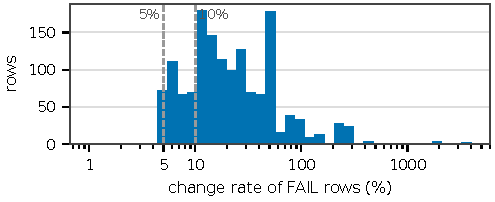
\includegraphics[width=\linewidth]{./figures/fig4-histogram.pdf}
\caption{全FAIL行(1,465行)の変動率分布(対数軸)．破線は既定閾値(detection 5\% / db 10\%)．日常変動の本体に対し，100\%超の構造イベント群が裾として分離する．FAIL中はcron再実行により同一イベントの行が繰り返し計上される点に注意．}
\label{fig:histogram}
\end{figure}

\subsection{チェックの相補性と検査の改良}
\label{sec:blindspots}

運用からは，チェック間の相補性と，検査自身の弱点の両方が見えた．
相補性の例がCVRF消失(\ref{sec:prevented}節の事例1)である．
DBチェックのKB比較はKBキーの集合しか見ないため，キー集合が不変のままCVEエントリが大量消失した本事例では0\%を返したが，観点の異なるDnが検知結果の激減として捕捉し公開を止めた．
単一の指標には盲点があり，それを補うのが多観点のチェックである(「KB 0\% $\neq$ 変化なし」は運用の警告事項として成文化した)．
一方，弱点として露呈し改良につながったものが2つある．
(1)ecosystem一括の変動率は大ソースが小ソースの異常を希釈した(ソース単位への細分化で対処)．
(2)overrideの系統間非対称が片系統だけの慢性FAILを生んだ(groomingで両系統を同時に見ることで対処)．
検査は一度作って終わりではなく，発動事例からのフィードバックで分解能と運用を継続的に改良する対象である．
なお(1)のソース単位化の効果は後半の観測窓で実測できた．
レポートがソース名を持つため，前半では「cpe」と一括りだった変動が，vulncheck-nist-nvd2(110行)，cisco-json(42行)，fortinet-csaf(17行)，fortinet-cvrf(10行)，paloalto-json(5行)，jvn-feed-rss(5行)のように分解され，target名からソースを推定する必要がなくなった．
\ref{sec:prevented}節で述べた「分解能不足で判定を誤りかけた」事例と同型の希釈は，後半の窓では観測されていない．

\subsection{運用コストの実態}
\label{sec:opscost}

run単位のFAILの50\%は土日に発生しているが，これは上流ではなく人間側の信号である．
promoteが平日日中にしか行われないため，金曜夕方以降のイベントが週末じゅう再FAILし続ける(週末滞留)．
fail sequenceの持続時間(中央値11h / p90 48h)は検査の検出性能ではなくオペレータの応答時間の分布を測っており，通知や承認フローの自動化余地を見積もる直接の根拠となる．

\subsection{開発プロセスに対する最終ガードレールとしての価値}
\label{sec:guardrail}

本検査の副次的だが実感の大きい価値として，パイプライン開発の最終防衛線としての機能がある．
ユニットテストやコードレビューが工程ごとのコードの正しさを検査するのに対し，データパイプラインの意味的な正しさは集約後の出力でしか観測できない．
実際，期間中に唯一捕捉されたコード起因の異常(表\ref{tab:attribution})は，型の取り違えでソート処理が欠落し出力順序が非決定になるバグで，コンパイルもテストも通過するが，rawの変更266ファイルに対しextracted 23,163ファイルという構造差分(drift 274.5\%)として顕在化し，公開阻止と修正PRに帰結した．
また運用上は，開発版に破壊的変更を先行投入し検査で影響規模を定量観測してから安定版へ降ろす，変更前からFAILを予期しその発現範囲が想定に閉じていることを混入なしの証拠として使う(\ref{sec:prevented}節のピン解除)，といった能動的な使い方も定着した．
この「作られ方に依存せず生成物を検証する」性質は，AIエージェントによるコード生成が開発の速度と量を押し上げる今後，コードレビューのスケール限界を補う出力レベルのガードレールとして重要性を増すと考える．
なお本運用では，発動時の一次調査(原因帰属)はAIエージェントに委ねる一方，その報告の検証と検査を通す判断(promote)は人間に限定している(\ref{sec:promote}節，\ref{sec:method}節)．
生成も調査も速く，検証は出力で，承認は人間で，という役割分担である．

\section{関連研究}
\label{sec:related}

\textbf{脆弱性データベースの品質}:
NVDをはじめとする脆弱性DBの品質は繰り返し測定されてきた．
CVE/NVDと外部レポート間の影響バージョン不整合の大規模検出\cite{dong19}，NVD，JVNDB，CNVDの登録プロセスとカバレッジの比較\cite{lin26}，NVDコーパスの品質監査と自動修正\cite{anwar22}，影響バージョン情報の実地検証\cite{nguyen13}，CVSS付与遅延の回帰分析\cite{ruohonen19}，NVD利用者の定性調査\cite{wunder24}などがある．
また，同一対象に対するスキャナやSCA(Software Composition Analysis)ツール間の検知結果の大きな不一致が，参照する脆弱性DBの差に相当程度帰着することも示されている\cite{imtiaz21,churakova25}．
2024年のNVD enrichment停滞は産業側の分析でも定量化された\cite{vulncheck24,anchore25}．
これらはいずれもフィードを外部から静的に(スナップショット間比較，コーパス監査，回顧的分析として)測定するものである．
本稿はこれに対し，測定器を本番の取り込み・公開パイプラインに常設し，フィード内容の経時変化そのものを下流消費者の視点で縦断観測した点で異なる．

\textbf{セキュリティデータフィードの品質測定}:
脅威インテリジェンスフィードについては，量，カバレッジ，遅延，正確性等の指標による比較測定が行われ，フィード間の重複の少なさや，消費者にとって品質が不可視であることが示されている\cite{li19,bouwman20,griffioen20}．
フィードの内容品質を測るという点で方法論的に本稿へ最も近い系譜だが，いずれも外部の研究として実施された横断測定である．
本稿は，単一フィードを自身の公開履歴と比較する縦断測定を，公開を保留する運用機構として常設した点が新しい．

\textbf{データパイプラインの検証}:
宣言的制約によるデータ品質検証\cite{schelter18,breck19}に加え，パイプライン自身の実行履歴から検証基準を自動導出する研究\cite{tu23,redyuk21}，新しいデータバッチが履歴から逸脱した際に下流のML再学習をブロックするゲート\cite{shankar23}があり，特に後者は「履歴との比較で公開・利用を止める」という意味論まで本稿と同型である．
テスト理論の観点では，本稿の検査は前公開版を比較対象(オラクル)とするdifferential testing\cite{mckeeman98}の時間軸変種，あるいはデータartifactに対する回帰テスト\cite{yoo12}の適用とみなせる．
これらとの差分は，(1)列統計ではなく検知結果と検知条件構造という意味レベルの差分を取ること，(2)セキュリティクリティカルな公開物を対象に，監査証跡付きのhuman-in-the-loop overrideを備えること，(3)検査の発動記録そのものを上流不安定性の測定データとして全数分析したこと，の3点である．

\textbf{国内の関連研究}:
国内では，脆弱性対策情報データベースJVNの提案\cite{terada05}に始まる脆弱性情報流通の系譜があり，近年は本トラックでOSSの脆弱性修正状況の収集と調査\cite{kuzuno24}，PSIRT向け脆弱性スクリーニング\cite{kanai24}など，公開脆弱性情報とその利用の間の乖離を扱う研究が続いている．
またIPAのJVN iPedia登録状況レポート\cite{ipa-jvnipedia}は，2024年のNVD公開遅延が国内DBの登録数を減少させたことを公式に記録しており，上流の不安定性が国内の脆弱性情報基盤へ波及する実例である．
一方，フィード内容の経時的不安定性を定量計測した国内の学術研究は，我々の調査の範囲では見当たらない．

\section{おわりに}
\label{sec:conclusion}

脆弱性DBの公開CIに公開前検査を実装し，116日間・943 runの全数調査を通じて，脆弱性情報の上流ソースの不安定性を69件の独立イベントとして定量観測した．
上流は消え，戻り，遡及的に書き換わり，アナウンスなく再編される．
しかもその大半は正当な変更である．
得られた知見は次の通りである．
(1)正常変動と異常イベントは変動率で概ね桁分離し，単純な閾値検査が実用になる．
ただし分解能(ソース単位)と閾値(対象単位のoverrideと定期grooming)は運用実績から継続的に導出する必要がある．
(2)発動原因の帰属は，収集・変換・構築の全工程が履歴管理されていることを成立条件とする．
前稿で報告した履歴管理基盤\cite{nakaoka2025}は，本測定と公開品質管理の土台として実証された．
本稿は同稿が課題として挙げた「差分の論理的な提示」「パイプラインの堅牢化」への，運用を伴う一つの回答でもある．
(3)FAIL時の復旧は「人間によるレポート確認+監査証跡付きoverride」として設計すべきである．誰が何を根拠に通したかが履歴に残ることが，安全ネットを緩める操作の正当性を支える．
(4)上流の恒久的劣化には，取り込みのピン留めや自らの取得履歴からの復元という出口が要る．
(5)生成物を出力レベルで検証する検査は，上流だけでなく自らの開発プロセスに対する最終防衛線としても機能し，テストとレビューをすり抜ける意味的バグの捕捉や，破壊的変更の影響範囲の定量確認に実際に寄与した．
コード生成にAIが入り込む開発形態において，この価値は今後増すと考える．

今後の課題として，fetch段階での欠損検出(月次ドキュメント丸ごと消失時にコミットしない等)，通知や承認フローの改善による週末滞留の解消，観測の長期蓄積による時系列特性(月次サイクル等)の統計的確立，および同一上流を消費する他エコシステムとの観測の突合が挙げられる．

\bibliographystyle{junsrt}
\bibliography{./refs.bib}

\end{document}
